\documentclass[output=paper]{LSP/langsci} 
\author{Katrin Hein\affiliation{Institut für deutsche Sprache, Mannheim}
}
\title{Modeling the properties of German phrasal compounds within a
  usage-based constructional approach}
\shorttitlerunninghead{Modeling German phrasal compounds within a
  constructional approach } 
\abstract{This paper discusses phrasal compounds in German (e.g. ``Man-muss-doch-über-alles-reden-können''-Credo,  ‘one-should-be-able-to-talk-about-everything motto’). It provides the first empirically based investigation and description of this word-formation type within the theoretical framework of construction grammar. While phrasal compounds pose a problem for ``traditional'' generative approaches, I argue that a usage-based constructional model (e.g. \citealt{Langacker1987}; \citealt{Goldberg2006}) which takes into consideration aspects of frequency provides a suitable approach to modeling and  explaining their properties. For this purpose, a large inventory of phrasal compounds was extracted from the \textit{German Reference Corpus} (DeRe\-Ko) and modeled as pairings of form and meaning at different levels of specificity and abstractness within a bottom-up process. 

Overall, this paper not only presents a new and original approach to phrasal compounds, but also offers interesting perspectives for dealing with composition in general.}
\ChapterDOI{10.5281/zenodo.885123}
\maketitle

\begin{document}
\section{Introduction}\label{sec:hein:1}

This paper discusses so-called ``phrasal compounds'' (PCs) (e.g. \textit{``Man-muss-doch-über-alles-reden-können''-Credo}, ‘one should be able to talk about everything mot-\linebreak to’) or \textit{``Second-Hand-Liebe''}, ‘second-hand love'), which can be defined as ``complex words with phrases in \isi{modifier} position” (\citealt[153]{Meibauer2003}; cf. \citealt[7]{Lawrenz2006}). They are largely ignored in the research literature, although the study of PCs is worthwhile in theoretical terms alone and sheds an important light on the process of composition in general.

\citet{Hein2011} has shown that this word-formation type poses a problem for ``traditional'' generative approaches which assume a modular architecture of grammar and do not allow for ``\isi{syntax} \textit{in} morphology''. And even the approaches which can handle the formal generation of PCs because they provide for a non-linear, i.e. a recursive, interaction between morphology and \isi{syntax}, fail to explain \textit{why} a speaker chooses a PC instead of a prototypical N-N-compound like \textit{Baumhaus} (‘tree house’).\footnote{An exception is \citet{Meibauer2007} who tries to give an explanation for the expressivity of PCs by adapting  \citegen{Levinson2000} ``Theory of Generalized Conversational Implicatures''. Moreover, Trips (e.g. \citealt{Trips2012,Trips2016}) provides an analysis of PCs within Jackendoff’s model of Parallel Architecture which allows her ``to gain further insights into the question of why PCs are built at all by speakers\slash writers and why they are sometimes preferred over other options” \citep[322]{Trips2012}.} 

This paper argues that a \isi{usage-based} \isi{constructional} model (e.g. \citealt{Langacker1987}; \citealt{Goldberg2006}) which entails direct pairings of form and meaning (``constructions'') and takes into consideration aspects of frequency, provides a suitable approach to modeling and explaining the properties of PCs. For this purpose, the findings of a broad empirical, construction-\isi{grammatical} investigation are presented. 

To gain new insights into the functioning of this word-formation type, I extracted a large number of \ili{German} PCs from the \textit{Deutsches Referenzkorpus} (DeRe\-Ko) (\citealt{IDS2011a}) in a first step. In a second step, an inventory of 1,576 individual nominal PCs was analyzed and modeled as pairings of form and meaning (``constructions'') at different levels of specificity and abstractness within a \isi{bottom-up process}. In addition, I will also relate the posited constructions within a so-called ``constructicon'' (e.g. \citealt[95]{ZiemLasch2013}) to each other. 

As neither an empirically based investigation nor a description of PCs within the theoretical framework of \isi{construction grammar} has been provided so far, I will present a new and original approach to the word-formation type that offers interesting perspectives for dealing with composition in general. 


\section{The bottom-up model}\label{sec:hein:2}
\subsection{Data -- empirical basis}\label{sec:hein:2.1}
The data for my study has been extracted from the \textit{\ili{German} Reference Corpus} (DeReKo) \citep{IDS2011a} which at that time comprised 5.4 billion words and ``constitutes the largest linguistically motivated collection of contemporary \ili{German} texts” \citep[2]{CLPA}. Therefore, this investigation is based on written text. While DeReKo contains fictional, scientific and newspaper texts as well, I concentrated only on newspaper texts.

\subsubsection{Data extraction}\label{sec:hein:2.1.1}
Technically speaking, the extraction of PCs from the corpus was done with the help of a perl script containing different types of regular expressions. This method has led to the extraction of 1,182,720 strings; as it is synonymous with searching for certain \textit{surface forms}, it is clear that the search results did not only contain PCs, but also a large number of word strings which only \textit{look like} PCs (e.g. street names consisting of three words with dashes between them). See \citet[Chapter~III.1]{Hein2015} for a detailed explanation of how PCs can be found and extracted from DeReKo and for an overview of the complete corpus that has been compiled for my study.

\subsubsection{Data selection and grouping}\label{sec:hein:2.1.2}
As the conducted \isi{bottom-up process} or rather the underlying analyses are very complex, it was not possible to consider every single genuine PC comprised in the results extracted from DeReKo. In fact, I worked with an inventory of 1,576 nominal PCs (types), arguing that this inventory can be seen as an acceptably representative sample of the potential spectrum of nominal phrasal compounding.\footnote{Only nominal PCs have been considered in the study. (See \citealp[Chapter~III.2]{Hein2015}) for a detailed description and a discussion of the analyzed inventory.}

What criteria were applied for the compilation of this inventory, i.e. the corpus of the study? First, I attempted to consider the widest possible range of PCs.  Second, I had to bear in mind the targeted \isi{bottom-up process}: In order to model the properties of the word formation pattern within a \isi{bottom-up process}, it is important to be able to work with different groups of compounds which share certain formal and\slash or semantic properties. As a starting point for compiling the corpus and its subgroups, I chose the properties of the head constituent.\footnote{\sectref{sec:hein:2.4} will explain why it is plausible to start from the properties of the head when compiling the corpus and its subgroups.} 

Overall, four different types of nominal heads \--- and consequently four main types of PCs -- were considered: 
\begin{enumerate}
\item PCs with a non-derived head noun; 
\item PCs with a deadjectival head noun; 
\item PCs with a \isi{desubstantival} head noun; 
\item PCs with a deverbal head noun. 
\end{enumerate} 
\textit{Within} those four main groups, I also tried to consider a variety of head constituents with different semantic\slash formal properties. This is why each main group of PCs is separated into several subgroups. Tables~\ref{tab:hein:1} to \ref{tab:hein:4} try to illustrate the principle of compiling different PC-groups and PC-subgroups according to the properties of the head. (Note that the following lists are not complete -- a detailed description of grouping and selecting the data can be found in \citealt[Part III]{Hein2015}).
 
\begin{table}
\begin{tabular}{p{3cm}p{8cm}}
\lsptoprule
 Subgroup\footnotemark{} & PC-examples\footnotemark{}\\
\midrule
 Concrete noun \newline(absolute) & \textit{Working-Class-Junge} (‘working-class boy')\footnotemark{}\newline
\textit{Jeans-und-T-Shirt-Mädchen}\newline
\textit{Zweite-Wahl-Obst} \\

\tablevspace
 Concrete noun\newline (relative)\footnotemark{} & \textit{No-name-Vater} (‘no-name father')\newline
 \textit{Kleine-Leute-Sohn}\newline
\textit{Take-That-Kollege}\\

\tablevspace
 Abstract noun for the description of a point of view & \textit{Entweder-Oder-Credo} (‘either-or motto')\newline
\textit{``Das-Boot-ist-voll{\textquotedbl}-Parole}\newline
\textit{``Wer-macht-den-meisten-Lärm''-Devise}\\
\lspbottomrule
\end{tabular}
\caption{ Group 1: PCs with a non-derived head noun}
\label{tab:hein:1}
\end{table}
\addtocounter{footnote}{-3}
\stepcounter{footnote}\footnotetext{Depending on the properties of the head.}
\stepcounter{footnote}\footnotetext{All the examples used in this study are taken from DeReKo (\citealt{IDS2011a}) and are cited in their original writing (hyphens, type and position of quotation marks, etc.). See \citealp[Chapter~III.2.2]{Hein2015} for a discussion of criteria linked to the PC-status (e.g. the underlying concept of phrases and sentences).}
\stepcounter{footnote}\footnotetext{In this as well as the following tables only the first example of each type of PC is translated into \ili{English}.}
\stepcounter{footnote}\footnotetext{For each PC-main-type I have tried to consider valent\slash relative and non-valent head nouns.}

\begin{table}
\begin{tabular}{p{3cm}p{8cm}}
\lsptoprule
 Subgroup{} & PC-examples\\
\midrule

Nomen Qualitatis & \textit{Mir-doch-egal-Leichtigkeit} (`I-don't-care ease')\newline
\textit{50er-Jahre-Naivität} \newline
\textit{Trinkmilchjoghurt-mit-Erdbeergeschmack--Rosa}\newline
\textit{Frau-Holle-Blau}\\
\tablevspace
 Denomination of a person & \textit{Formel-1-Liebling} (‘Formula 1 favorite')\newline
\textit{``Im-fremden-Bett-schlaf-ich-immer-schlecht-Sensibelchen''}\\
\tablevspace
 Valent noun & \textit{Prinz-Harry-Besessenheit} (‘Prince Harry obsession')\newline
\textit{Zwölf-Minuten-Länge}\\
\lspbottomrule
\end{tabular}
\caption{Group 2: PCs with a deadjectival head noun}
\label{tab:hein:2}
\end{table}

\begin{table}
\begin{tabular}{p{3cm}p{8cm}}
\lsptoprule
 Subgroup & PC-examples\\
\midrule
 Denomination of  a person & \textit{High-Society-Fräulein} (‘high-society lady’)\newline
 \textit{``Morgens-Fango/Abends-Tango-Rentner{\textquotedbl}}\newline
\textit{Bad-Taste-Komiker}\\

\tablevspace
 Collective noun & \textit{Zwei-Klassen-Menschheit} (‘two-class mankind')\newline
\textit{Vor-68er-Studentenschaft}\\

\tablevspace
 Relative noun & \textit{Ost-West-Freundschaft} (‘East-West friendship')\newline
 \textit{Cosa-Nostra-Häuptling}\newline
\textit{Schütze-des-Fünf-zu-null-Mutti}\\
\lspbottomrule
\end{tabular}
\caption{ Group 3: PCs with a desubstantival head noun}
\label{tab:hein:3}
\end{table}

\begin{table}
\begin{tabularx}{\textwidth}{lQ}
\lsptoprule
 Subgroup & PC-examples\\
\midrule
 Nomen Agentis & \textit{Tour-de-France-Kenner} (‘Tour-de-France expert')\newline
\textit{Rote-Rosen-Verkäufer} \newline
\textit{Immer-mal-wieder-Raucher}\\
\tablevspace
 Nomen Loci & \textit{Dreieinhalb-Zimmer-Bleibe}\newline (‘three-and-a-half-room apartment')\newline
\textit{60er-Jahre-Siedlung}\\

\tablevspace
 Nomen Actionis &  \textit{Heile-Welt-Bedürfnis} (‘rosy-world desire')\newline
\textit{``Dumme-Jungen-Gequatsche{\textquotedbl}}\newline
\textit{``Null Bock{\textquotedbl}-Verhalten}\newline
 \textit{Ich-habe-es-ja-gesagt-aber-ihr-habt-nicht-auf-mich-gehört-Gerede}\\

\tablevspace
 Nomen Acti & \textit{Kain-und-Abel-Tat} (‘Cain-and-Abel deed')\newline
\textit{``Habemus Papam{\textquotedbl}-Rede} \\
\lspbottomrule
\end{tabularx}
\caption{Group 4: PCs with a deverbal head noun}
\label{tab:hein:4}
\end{table}

\subsection{Scheme of analysis}\label{sec:hein:2.2}
To understand the \isi{bottom-up process}, not only is the arrangement of the data (cf. the previous \sectref{sec:hein:2.1}) important, but also the scheme of analysis which was used to classify the PCs from the corpus and to describe them as pairings of form and meaning requires a brief explanation.\footnote{In this paper I can only give a brief \textit{simplified} overview over the categories I used. Cf. \citet[Chapter~III.2.2]{Hein2015} for a more elaborated description.}

Overall, a variety of formal and semantic properties of PCs is involved, e.g. syntactic and pragmatic properties of the nonhead constituent, valence properties of the head constituent as well as the semantic relation between the two constituents, i.e. the semantic role adopted by the nonhead. Many of these properties are also relevant for the description of prototypical compounds like \textit{Baumhaus} (‘tree house') -- thus the innovativeness of my approach is not caused by creating completely new categories, but by the way those categories are combined with each other. 

In accordance with the theoretical background of my work -- i.e. the construction \isi{grammatical} framework -- PCs are described as direct pairings of form and meaning.\footnote{Note that my study is based on a wide understanding of meaning which includes semantic aspects as well as pragmatic aspects. This is in line with the construction \isi{grammatical} rejection of the strict separation between semantics and pragmatics (cf. \citealt[123]{Kay1997}).} This is why the levels and categories of analysis are divided into two groups: properties for the description of the form side vs. properties for the description of the meaning side of PCs. Tables~\ref{tab:hein:5} and \ref{tab:hein:6} list the levels of analysis in accordance with this distinction and give some \textit{examples} for corresponding categories and PCs.

\begin{table}
\begin{tabularx}{\textwidth}{>{\raggedright}p{3cm}>{\raggedright}p{3.5cm}Q}
\lsptoprule
Level of analysis & Category (examples) & PC (examples)\\
\midrule
 Syntactic properties of the nonhead &  Phrase\_NP& 
\textit{Sechseinhalb-Tage-Woche} (‘six-and-a-half-day week’); \textit{Harte-Jungs-Gerede; Söhne-Mannheims-Jahr;}\\
 
 & Sentence\_declarative \newline …  &   \textit{Ich-esse-alles-Geplapper}  (‘I-eat-everything talk') \\ \tablevspace
 
 Phraseological properties of the nonhead &  Lexicalized\newline
					    freely formed\newline
					    … & 
					       \textit{Tour-de-France-Monat} \newline     
						\textit{Schmeiß-keine-Plastiktüten-in-den-Wald-Gerede}\\

\tablevspace
 Pragmatic properties of the nonhead &  = Communicative minimal unit \newline
					  (in the sense \citealt[86]{ZifonunEtAl1997}) & \textit{Alles-oder-Nichts-Devise} (‘all-or-nothing slogan'); \textit{``Soldaten sind Mörder{\textquotedbl}-Jahr} \\
 & ≠ Communicative minimal unit & \textit{``Zwei-Minuten-Sache{\textquotedbl}} (‘two-minute affair')\textit{; Kaffee-und-Kuchen-Rentner}\\

\tablevspace
 Valence properties of the head &  valent\slash relational & \textit{Ost-West-Freundschaft} (‘East-West friendship'); \textit{Stop-and-Go-Tauglichkeit}\\
 
 
  & non-valent\newline  … & \textit{60er-Jahre-Siedlung} (‘1960s-housing')\\    
\lspbottomrule
\end{tabularx} 
\caption{Description of the \textit{form side} of PCs} 
\label{tab:hein:5}
\end{table}

\begin{table}
\begin{tabularx}{\textwidth}{p{3cm}lQ}
\lsptoprule
Level of analysis & Category (examples) & PC (examples)\\

\midrule \multirow{2}{3cm}{%
 Semantics~(1): How can the meaning of the PC be accessed? / Is its interpretation influenced by valence properties of the head?} & { Synthetic compound} 
		 & \textit{Zehn-Minuten-Länge} (‘ten-minute\newline  duration'); \textit{Alles-mögliche-Verkäufer}\newline  \textit{Last-Minute-Verkäufer} (`last-minute seller') \\
 & { Non-synthetic  compound} & \textit{Lange-Frisch-Milch}\\
\\\tablevspace

 \multirow{4}{3cm}{Semantics~(2):  Specific description of the relation between the two constituents and the role taken by the nonhead} & 
      1) subject-orientated\footnotemark & 1) \textit{Ein-Mann-Zuständigkeit} (‘\textit{one-man responsibility}') (Agens)\\
      & 2) object-orientated &  2) \textit{``Ernte 23{\textquotedbl}-Raucher} (‘\textit{Ernte 23 smoker}') (Patient)\\
      & 3) \isi{adverbial} & 3) \textit{Drei-Wochen-Mit\-glied\-schaft} (‘three-month membership') (temporal); \textit{Auf-der-Bank-Schläfer} (local);\\
      & 4) attribute-like & 4) \textit{``Pretty Woman{\textquotedbl}-Phänomen} (‘pretty-woman phenomenon') (theme); \textit{200-Häuser-Siedlung} (constitutional); \textit{Trinkmilchjoghurt-mit-Erdbeergeschmack-Rosa} (comparative); ``Früher-war-alles-besser{\textquotedbl}-Gerede (explicative) \\	    
	    
\lspbottomrule
\end{tabularx}
\caption{Description of the \textit{meaning side} of PCs}
\label{tab:hein:6}
\end{table}
\footnotetext{The specific semantic relations\slash roles are divided into four more abstract groups (``rough patterns'') which \citet[ 36 f.; 118 ff; 184]{Eichinger2000} developed for prototypical N-N-compounds. I will refer to those abstract groups in \sectref{sec:hein:3.1}. A detailed description of the assignment of semantic roles\slash relations to those abstract groups can be found in \citet[Chapter III.2.2.2.2]{Hein2015}.}


\subsection{Theoretical assumptions}\label{sec:hein:2.3}
As noted above, the aim of my study is to model the properties of PCs within a \isi{usage-based} \isi{constructional} approach. For these purposes, the 1,576 PC-types of the corpus (cf. \sectref{sec:hein:2.1}) are modeled as constructions at different levels of specificity and abstractness within a \isi{bottom-up process}. Which theoretical assumptions are crucial for this undertaking?



The basic idea for my approach is formed by Booij’s (\citeyear{Booij2010}: 3) observation ``that word formation patterns can be seen as abstractions over sets of related words''. This means that complex words -- like PCs -- are licensed by abstract schemata\slash patterns. Between a complex word and the scheme that allows for its formation, a relation of ``instantiation'' is assumed. 



More\-over, it is important to underline that I adopt the central assumption of \isi{usage-based} theories that frequency aspects have an influence on the development of such abstract patterns (e.g. \citealt[38]{ZiemLasch2013}). This assumption is, among others, based on the psychological phenomenon of ``entrenchment'' that refers to the development of ``cognitive routines'' \citep[130]{Langacker1988}: ``The occurrence of psychological events leaves some kind of trace that facilitates their re-occurrence. Through repetition, even a highly complex event can coalesce into a well-rehearsed routine that is easily elicited and reliably executed.'' Therefore, a linguistic structure that is ``pre-packaged'' because of  its entrenchment can be perceived as a holistic unit (\citealt[3f]{Langacker2000}).



According to the significance ascribed to frequency, I adopt Goldberg’s (\citeyear[5]{Goldberg2006}) definition of the notion ``construction'' in which non-predictability is not the only crucial criterion anymore:\footnote{Cf. \citet[Chapter~II.2]{Hein2015} for a detailed discussion of different definitions for the notion of construction and their applicability for PCs.}


\begin{quote}
Any linguistic pattern is recognized as a construction as long as some aspect of its form or function is not strictly predictable from its component parts or from other constructions recognized to exist. In addition, patterns are stored as constructions even if they are fully predictable as long as they occur with sufficient frequency. 
\end{quote}


The extent to which the pattern ``phrasal compounding'' fulfills this criterion of frequency and productivity (cf. \citealt[51f]{Booij2010}) has been shown in \citet{Hein2015}\footnote{To what extent PCs fulfill the criterion of non-predictability is discussed in \citet[Chapter~II.2.2.3]{Hein2015}.}: While it is only \textit{theoretically hypothesized} in the literature that phrasal compounding is a productive word formation pattern (c.f. \citealt{Lieber1992}, \citealt{Meibauer2003}), I conducted an empirical study to check whether PCs have hapax-status in my corpus. The latter is a productivity measure proposed by \citet{Baayen1992}; so-called ``hapax legomena'' are defined as the ``the number of once-words'' \citep[28]{Tuldava2005} within a specific textual context. This measure indicates if ``the language user comes across new types from time to time” (\citealt[52]{Booij2010}; cf.  \citealt[106]{ZiemLasch2013}). 

The results of my productivity study can only be presented briefly at this point (cf. \citealt[Chapter III.3.2]{Hein2015} for the complete study): Counting the absolute frequencies of the 1,576 PC-types from the corpus, i.e. counting the number of tokens for each type in the corpus, showed that 75\% have the status of hapaxes. Although 25\% of the PC-types occur more than once in my corpus, one can conclude that phrasal compounding is a productive word formation pattern for two reasons: Taking a closer look at the words which occur more than once in my corpus shows that among them are many completely lexicalized forms like \textit{35-Stunden-Woche} (‘35-hour week’) (4.485 tokens) -- it should be clear that completely lexicalized PCs can’t be ``new types''. Moreover, the high frequency types do not have a large scattering across different head nouns (here again, a dominance of the head noun \textit{Woche} can be stated).

All in all, the empirical investigation of productivity indicates that it is plausible to ascribe the theoretical status of a construction to the general pattern ‘phrasal compounding’ within a \isi{usage-based} \isi{constructional} approach. 


\subsection{Modeling of the data}\label{sec:hein:2.4}
Finally, I will show how the empirically gained data and its subcategorization, the scheme of analysis and the theoretical assumptions work together in the \isi{bottom-up process}.


Generally speaking, the \isi{bottom-up process} takes the 1,576 individual complex words as a starting point. At first, each of them is described as a direct pairing of form and meaning properties, applying the scheme of analysis that has been explained in \sectref{sec:hein:2.2}. I then attempt to make generalizations across groups of PCs that share some of the crucial formal\slash semantic properties of their head constituent (cf. \sectref{sec:hein:2.1.2}). The underlying wor\-king hypothesis is that PCs with an identical or formal\slash semantic comparable head possess commonalities on their meaning side which can be captured via constructions. This hypothesis is plausible insofar as the head is crucial for the basic semantic interpretation of \isi{determinative} compounds (e.g. \citealt[38]{Fandrych1994}) in general.\footnote{From my point of view, it is beyond doubt that PCs are word formation products, i.e. genuine compounds (cf. \citealt[12]{Schlücker2012} for a comparable argumentation).} At this point it becomes clear why the properties of the head were chosen as a starting point for the compilation of different PC-subgroups (cf. \sectref{sec:hein:2.1}) in my study. 

On the one hand, the procedure sketched out allows me to posit a variety of semantically orientated sub-constructions. On the other hand, I will try to stipulate an abstract construction for the word-formation type by generalizing about the posited sub-constructions. This means that at the highest point of the \isi{bottom-up model}, an abstract representation for phrasal compounding is carved out on the basis of the individual words and the generalizations that are possible within the PC-main-groups and the PC-subgroups. 



According to the theoretical assumptions which have been discussed in the previous section (cf. \sectref{sec:hein:2.3}), it is important to underline that aspects of frequency play an important role for the identification of strong form-meaning-correlations in the data.  Therefore in this study, constructions are only posited for such correlations which occur with a sufficient frequency.\footnote{In consideration of the fact that ``real language'' is characterized by variation and special cases, the applicability of this ``frequency criterion'' is not always easy. In short, it’s the question of what can count as ``enough frequent'' to stipulate a construction which is crucial here. Cf. \citet{Hein2015} for a critical discussion of the applicability of this frequency criterion on authentic data.} As becomes evident in \sectref{sec:hein:3}, the absolute frequency is not the only aspect crucial in this context. In addition, the productivity of observable form-meaning-correlations has to be considered (i.e.: Are certain patterns limited to a very special type of head noun, or are they instantiable for different types of heads?).  



What does the concrete application of the process described above look like? After the division of the corpus data into the four main groups (non-derived vs. de-\isi{adjectival} vs. \isi{desubstantival} vs. deverbal head, cf. \sectref{sec:hein:2.1.2}), all PCs with the same lexeme in head position (e.g. all PCs with the head noun \textit{Rot}) are analyzed according to the scheme of analysis sketched out in \sectref{sec:hein:2.2} in a first step. In doing so, similarities on the meaning side can be carved out and captured within more abstract generalizations. 



In a second step, this procedure is transferred to groups of PCs with a semantically similar head noun (e.g. all PCs with a nonhead describing a color \slash  all PCs with a Nomen Qualitatis head). In a third step, I am trying to generalize over \textit{all} members of one main group (i.e. all PCs with a de-\isi{adjectival} nominal head). This means that I am asking whether all PCs from one main group display a) generalizable commonalities and b) display certain distinctive form-meaning-correlations that are characteristic for this special group. 



The fourth -- and last -- step is to explore whether it is possible to stipulate one (or more) form-meaning pairings that can likewise display the properties of \textit{all} PCs from my corpus. 


\section{Results}\label{sec:hein:3}

In this section, the main \textit{results} of the \isi{bottom-up process} described in the previous section are carved out. First of all, it is important to underline that it was indeed possible to structure the empirically gained, broad inventory of 1,576 PCs with the help of pairings of form and meaning at varying degrees of abstraction (cf. \sectref{sec:hein:4} for theoretical implications of this finding). Due to the lack of space, I cannot provide a complete reproduction of all results gained in \citet{Hein2015}.  Rather, I will focus on three main aspects: First, I will present some central universal patterns of phrasal compounding (\sectref{sec:hein:3.1}). In this context, I will discuss quite specific constructions as well as more abstract constructions.  Moreover, the most central representation for the pattern phrasal compounding is carved out (\sectref{sec:hein:3.2}). Finally, I will sketch out how the stipulated constructions can be related to each other (\sectref{sec:hein:3.3}).


\subsection{Universal patterns of phrasal compounding} \label{sec:hein:3.1}
\subsubsection{Fine-grained generalization}\label{sec:hein:3.1.1}

The corpus-based investigation points out that there are various, non-restricted possibilities concerning the meaning side of PCs: All the semantic roles\slash relations (cf. the examples in table 6) which  play  a role for prototypical \isi{determinative} compounds like \textit{Baumhaus} (`tree house') seem to be instantiable in the pattern ``phrasal compounding'', too.\footnote{The form side of nominal PCs is likewise principally open. My investigation clearly shows that phrasal compounding is open to all types of phrases\slash sentences in nonhead position (cf. \citealt[Chapter III.3.1.2]{Hein2015}).}  At the same time, it becomes apparent that there are a very limited number of specific meaning types which can be labeled as particularly universal\slash established for phrasal composition. Being universal\slash es\-ta\-blished is justified in two respects within a \isi{usage-based} approach: First, in the corpus there are a high number of concrete instantiations for the patterns listed below. Second, those patterns of meaning are productive insofar as there are no or almost no restrictions for their instantiation. This means that those meaning patterns are not limited to constituents with very specific properties.  

Talking about universal patterns of phrasal compounding under the perspective of fine-grained generalization, the reading ``explicative'' has to be mentioned in the first place. Crucial for this pattern is the complete (semantic) spelling out of the constituent B through the constituent A. For example, \textit{Alles-oder-Nichts-Devise} (`all-or-nothing slogan’) is a Devise which is characterized by the attitude ‘Alles oder nichts’. \figref{fig:hein:1.1} illustrates how the formal and semantic properties of the PCs with a corresponding reading can be captured via a construction:
 
\begin{figure}\raggedright
\begin{framed}
\caption{Explicative-Construction\label{fig:hein:1.1}}
\noindent \textbf{Explicative-Construction}\\
\noindent [[Sentence/Sentence-ellipt /Sentence-Scheme-ellipt /Verb Group\textsubscript{+CM}/Phrase\textsubscript{+CM}]\textsubscript{{}-Proper Name} -- [Substantive]\textsubscript{+/-valent} ]\textsubscript{N; PC}\\
\vspace{\baselineskip}
\noindent
e.g. \textit{Alles-oder-Nichts-Devise} (‘all-or-nothing slogan')\\
\textit{``Im-fremden-Bett-schlaf-ich-immer-schlecht-Sensibelchen''}\\
\textit{``Schaun-wir-mal-Franz{\textquotedbl} }\\
\textit{``Zu mir oder zu dir{\textquotedbl}-Gequatsche}\\
\textit{Wer-kriegt-wen-Albernheit}\\
\textit{Coca-Cola-trink-Unterhaltungs-Freundschaft}\\
\textit{Work-in-Progress-Dings}\\
\textit{Zurück-zu-den-Grundsätzen-Rede}\\
\textit{Keine-Drogen-Geschwätz}\\
\textit{Sowohl-Als-auch-Ver\-hal\-ten}\\
\textit{Ich-will-mir-was-Gutes-Tun-Bedürfnis}\\
\textit{``Vater ist der Beste{\textquotedbl}-Stolz}\\
\textit{Is-was?-Dreistigkeit}
\end{framed}
\end{figure}

\largerpage[2]
This reading becomes manifest in PCs whose first constituent is an entire sentence (e.g. \textit{Ich-will-mir-was-Gutes-Tun-Bedürfnis}, ‘I-want-to-do-something-good-for-me need’), an elliptical sentence (\textit{``Zu mir oder zu dir{\textquotedbl}-Gequatsche}, ‘To-me-or-to-you talk’), an elliptical sentence scheme (e.g. \textit{Sowohl-Als-auch-Ver\-hal\-ten}, ‘both-sides-of-the-coin behavior’), a verb group in the sense of \citet{ZifonunEtAl1997} (e.g. \textit{Coca-Cola-trink-Unterhaltungs-Freundschaft}, ‘Coca-Cola-drinking-\linebreak discussion friendship’) or a phrase which has the status of a communicative minimal unit (CM) (e.g. \textit{Keine-Drogen-Geschwätz}, ‘no-drugs talk’).\footnote{Cf. \citet[Chapter~III.2.2.1.2]{Hein2015} for an explanation of the underlying phrase concept.} 

Moreover, this reading occurs in \textit{all} four main groups (cf. \sectref{sec:hein:2.1.2}), i.e. in PCs whose second constituent is a non-derived noun (e.g. \textit{``Schaun-wir-mal-Franz{\textquotedbl}}, ‘let's-see-what-happens Franz’), a deadjectival noun (\textit{{\textquotedbl}Vater ist der Beste{\textquotedbl}-Stolz}, ‘father-is-the-best pride’), a \isi{desubstantival} noun (\textit{Coca-Cola-trink-Unterhaltungs-Freundschaft}) or a deverbal noun (\textit{Sowohl-Als-auch-Verhalten}). This variety of formal types linked to an explicative reading underlines the productivity of the pattern. The cognitive plausibility of the form-meaning pair stipulated in \figref{fig:hein:1.1} is also strengthened by the fact that 331 of the 1,576 PCs from my corpus are instantiations of this construction; only the reading ``theme'' (cf. \figref{fig:hein:1.3}) is more frequent in my investigation. Moreover, the Explicative-Construction is a very strong construction insofar as it displays an \textit{inevitable} correlation between form and meaning, e.g. all PCs with the illustrated form have an explicative meaning.  In my investigation, this is a unique feature of the Explicative-Construction. 

There are two more specific readings which occur in all four main groups, i.e. which are not restricted to specific types of head nouns and can therefore be labeled as universal patterns of phrasal compounding: the reading ``domain'' and the reading ``theme''. Instead of an inevitable form-meaning correlation, the corresponding constructions in Figures~\ref{fig:hein:1.2} and \ref{fig:hein:1.3} display form-meaning correlations which can be regarded as very probable if one considers aspects of frequency and productivity.

The reading ``domain'' is characterized by the creation of a reference field for the head noun B through the first constituent A and occurs 205 times in the corpus. Its form side is converse to the form side of the Explicative-Construction: It is limited to phrases without CM-status and sentences that are proper names.

\begin{figure}
\begin{framed}\raggedright
\caption{Domain-Construction\label{fig:hein:1.2}}
\noindent \textbf{Domain-Construction}\\
\noindent [[Phrase\textsubscript{{}-CM}/Sentence\textsubscript{+Proper Name}] -- [Substantive]\textsubscript{+/-valent}]\textsubscript{N;} \textsubscript{PC}\\
\vspace{\baselineskip}
\noindent
e.g. \textit{Upper-Class-Mädchen} (‘upper-class girl')\\
\textit{Tour-de-France-Woche}\\
\textit{Berlin-Mitte-Phänomen}\\
\textit{Take-That-Kollege}\\
\textit{``Big-Brother''-Liebling}\\
\textit{Kopf-Rumpf-Länge}\\
\textit{Au-pair-Fräulein}\\
\textit{Trimm-Dich-Verhalten}
\end{framed}
\end{figure}


The semantic reading ``theme'' is the most frequent reading in the corpus (405 instantiations) and is characterized by the slogan-like spelling out of a communicative or artistic concept in B through the first constituent A.

\begin{figure}
\caption{Theme-Construction\label{fig:hein:1.3}}
\begin{framed}\raggedright
\noindent \textbf{Theme-Construction}\\
\noindent [[Phrase\textsubscript{{}-CM}/Infinitive-coordinated/Verb Group\textsubscript{{}-CM} /Sentence\textsubscript{+Proper Name}] -- [Substantive]\textsubscript{+/-valent}]\textsubscript{N;} \textsubscript{PC}\\
\vspace{\baselineskip}
\noindent 
e.g. \textit{Happy-Mosel-Jahr} (‘Happy Mosel Year’)\\
\textit{``La Bohème{\textquotedbl}-Jahr}\\
\textit{Don-Quijote-Sujet}\\
\textit{Kosten-Nutzen-Devise}\\
\textit{``Holy-Bandits{\textquotedbl}-Motto}\\
\textit{Vorher-nachher-Peinlichkeit}\\
\textit{Wild-West-Sportler}\\
\textit{Wald-und-Wiesen-Italiener}\\
\textit{Fast-Food-Zeugs}\\
\textit{Achse-des-Bösen-Rede}\\
\textit{``Stop-and-Go{\textquotedbl}-Verhalten}\\
\textit{``Hilfe-Such-Verhalten{\textquotedbl}}
\end{framed}
\end{figure}

\subsubsection{Coarse-grained generalization}\label{sec:hein:3.1.2}
At the center of this section are universal patterns of phrasal compounding that are gained through coarse-grained generalization over the observable form-mean\-ing correlations in the corpus. 


They can be understood as the result of generalizing over the more specific form-meaning correlations of the type presented in the previous section.  While the meaning side of the constructions in Figures~\ref{fig:hein:1.1} to \ref{fig:hein:1.3} was described with the help of specific semantic relations\slash roles, I will work with more abstract semantic descriptions below: As already mentioned in \sectref{sec:hein:2.2} (``scheme of analysis''), I assign the specific semantic relations\slash roles to four more abstract groups (``rough patterns'') that \citet[36 f.; 118 ff.; 184]{Eichinger2000} developed for prototypical compounds: 
\begin{enumerate}
\item subject-orientated patterns; 
\item object-orientated patterns;  
\item \isi{adverbial} patterns; 
\item attribute-like patterns.
\end{enumerate}

Two questions are crucial in this context: Is there a distinguishing abstract pattern for each of the four main groups of PCs, i.e. is it crucial for the meaning side if the head-noun is non-derived, deadjectival, \isi{desubstantival} or deverbal? And which of Eichinger’s ``rough patterns'' can count as the most established pattern for phrasal compounding?

First of all, it has to be emphasized that there are instantiations for all four ``rough patterns'' in the corpus of this investigation\footnote{For example, the Explicative-Construction stipulated in \figref{fig:hein:1.1} is an instantiation of the more abstract Attribute-like-Construction.} -- as already stated in \sectref{sec:hein:3.1.1}, phrasal compounding is open for the realization of all semantic relations that one can find in prototypical \isi{determinative} compounds. Thus, the following form-meaning correlation has to be stated at the highest point of the \isi{bottom-up model}:  


\begin{figure}
\caption{Subject-orientated - / Object-orientated - / Adverbial - / Attribute-like -Construction\label{fig:hein:1.4}}
\begin{framed}\raggedright
\textbf{Subject-orientated - / Object-orientated - / Adverbial - / Attribute-like -Construction}\\
\noindent
[[Syntagma] -- [Substantive]]\textsubscript{N;} \textsubscript{PC; +/-SynthC}\footnotemark
\end{framed}
\end{figure}\footnotetext{``SynthC'' is used as abbreviation for ``\isi{synthetic compound}''.}

While the pattern in \figref{fig:hein:1.4} illustrates all \textit{potentially formable}  meaning-types of PCs, the realization of one semantic pattern \--- attribute-like -- has to be labeled as particularly likely and universal.  This becomes clear when one looks at the frequencies in the corpus: 1,315 of the  1,576 PC-types are instantiations of the ``rough pattern'' attribute-like. However, the attribute-like-reading is not only frequent, but also productive insofar as there seem to be no restrictions for its instantiation: It is instantiated in all four main groups, i.e. this reading occurs for all types of nominal heads. Moreover, it is also the most frequent reading when one looks at the four subgroups separately. Last but not least, there are instantiations of this pattern in each single subgroup (e.g. concrete vs. abstract noun etc.) within the four main groups (cf. the description of data grouping in \sectref{sec:hein:2.1.2}).  All in all, those observations about the frequency, the productivity and the balanced distribution of this ``rough pattern'' within the corpus make it plausible to stipulate the following construction:

\begin{figure}
\caption{Attribute-like-Construction\label{fig:hein:1.5}}
\begin{framed}\raggedright
\textbf{Attribute-like-Construction}\\[1.5\baselineskip]
\begin{tabularx}{\linewidth}{lX}
\textbf{Form} & [[Syntagma] -- [Substantive]\textsubscript{non-derived,} \textsubscript{de-\isi{adjectival},} \textsubscript{de-substantival} \textsubscript{or de-verbal;} \textsubscript{+/-valent}] \textsubscript{N;} \textsubscript{PC} \\
\textbf{Meaning} & Comprises semantic relations/roles like ``domain'', ``explicative'', ``theme'', ``constitutional'' etc.\\
\end{tabularx}
\vspace{\baselineskip}\par
e.g. \textit{Wild-West-Sportler} (‘wild-west athlete')\\
\textit{``Im-fremden-Bett-schlaf-ich-immer-schlecht-Sensibelchen''\\
Is-was?-Dreistigkeit\\
Take-That-Kollege}\\
\textit{Zweite-Wahl-Obst}
\end{framed}
\end{figure}


With the lowest probability, the rough pattern ``\isi{adverbial}'' becomes manifest in PCs:  The corpus comprises only 50 types with this reading. Moreover, \isi{adverbial} readings occur only in two of the four main groups in exemplary fashion, i.e. with sufficient frequency and balanced distribution. As can be seen in \figref{fig:hein:1.6}, my investigation points out that an \isi{adverbial} relation between the two constituents is predominantly restricted to PCs with \isi{desubstantival} or deverbal nominal head.\footnote{This doesn’t mean that there is absolutely no evidence for PCs with an \isi{adverbial} reading and a non-derived or de-\isi{adjectival} head noun. Rather the number of such cases is so rare that it is not justifiable within a usage-based-approach to integrate this possible correlation into a representation that raises the claim to reflect established form-meaning correlations.}  The construction in \figref{fig:hein:1.6} is also less universal than the construction in \figref{fig:hein:1.5} insofar as \isi{adverbial} readings are restricted to a few quite specific semantic heads within the two main groups ``\isi{desubstantival}'' and ``deverbal''.

\begin{figure}
\caption{Adverbial-Construction\label{fig:hein:1.6}}
\begin{framed}\raggedright
\textbf{Adverbial-Construction}\\[1.5\baselineskip]
\begin{tabularx}{\linewidth}{lX}
\textbf{Form} & [[Phrase] -- [Substantive]\textsubscript{de-substantival/deverbal}]\textsubscript{N;} \textsubscript{PC; +/-SynthC}\\
\textbf{Meaning} & Comprises semantic relations/roles like ``temporal'', ``local'', ``causal'' etc.\\
\end{tabularx}
\vspace{\baselineskip}\par
e.g. \textit{Drei-Wochen-Mitgliedschaft} (‘three-week membership’)\\
\textit{Open-Air-Schläfer}
\end{framed}
\end{figure}

Though the form-meaning pairing is not completely universal, its status as a construction is supported by a very distinct, homogeneous form side -- only phrases, but no sentences can occur in the non-head position. 

What conclusions can be drawn from the \isi{bottom-up model} about the instantiation of subject- and object-orientated semantic patterns? 

At first glance, subject-orientated readings seem to be quite common in phrasal compounding: With 128 corresponding PCs, subject-orientated readings occur at the second-most in the corpus, followed by object-orientated readings with 83 corresponding PCs. As it is assumed that in \isi{determinative} compounds the exploitation of the subject-position is less common than the exploitation of the object-position as a matter of principle (cf. \citealt[131]{Eichinger2000}), this is a surprising finding. But a closer look at the results shows that the frequency of subject-oriented readings is caused by a high-frequent occurrence in two specific subgroups within the main group ``non-derived noun'' (abstract nouns which describe a point of view; relational concrete nouns). For this reason, the frequency of subject-orientated readings in my corpus should not be overrated.



Nonetheless, subject-orientated readings occur in all four main groups, i.e. there are no restrictions for the head-noun. However, as represented in \figref{fig:hein:1.7}, PCs with a subject-orientated reading predominantly exhibit a \textit{valent} head noun, i.e. a head noun which has a clearly agentive component (e.g. \textit{Maxime} in \textit{Blaue-Reiter-Maxime}, ‘Blaue-Reiter maxim’). 

\begin{figure}[t]
\caption{Subject-orientated-Construction\label{fig:hein:1.7}}
\begin{framed}\raggedright
\textbf{Subject-orientated-Construction}\\[1.5\baselineskip]
\begin{tabularx}{\linewidth}{lX}
\textbf{Form} & [[Syntagma]\textsubscript{{}-CM} -- [Substantive]\textsubscript{+valent/agentive}]\textsubscript{N;} \textsubscript{PC; +/- SynthC} \\
\textbf{Meaning} & Comprises semantic relations/roles like ``Agens'', ``Experiencer'', ``Possessor'' etc.\\
\end{tabularx}
\vspace{\baselineskip}\par
  e.g. \textit{Vater-Sohn-Freundschaft} (‘father-son friendship')\textit{\\
 Ein-Mann-Zuständigkeit}
\end{framed}
\end{figure}


The instantiation of the object-orientated pattern is blocked for PCs with a non-derived head noun in my study, while it is very rare (only 3 corresponding forms in the corpus) in PCs with \isi{desubstantival} head nouns. This explains why in \figref{fig:hein:1.8} the object-orientated pattern is correlated to compounds with deadjectival or deverbal head noun. In other words, this meaning predominantly occurs in PCs whose head noun is not an ``originary substantive'' (cf. \citealt[235]{Hölzner2007}). Considering the valence properties of this type of nouns, this outcome is to be expected.  

\begin{figure}[t]
\caption{Object-orientated-Construction\label{fig:hein:1.8}}
\begin{framed}\raggedright
\textbf{Object-orientated-Construction}\\[1.5\baselineskip]
\begin{tabularx}{\linewidth}{lX}
\textbf{Form} & [[Syntagma]\textsubscript{{}-CM} -- [Substantive]\textsubscript{de-\isi{adjectival}/}\textsubscript{deverbal;} \textsubscript{+valent}]\textsubscript{N}\textbf{\textsubscript{;}} \textsubscript{PC;} \textsubscript{SynthC}\\
\textbf{Meaning} & Comprises semantic relations/roles like ``Patient'', ``Co-Patient'', ``Stimulus'' etc. \\
\end{tabularx} 
\vspace{\baselineskip}\par
e.g. \textit{Rote-Rosen-Verkäufer} (‘red-roses seller’)\\
\textit{``Don Quichotte{\textquotedbl}-Dichter}
\end{framed}
\end{figure}

In conclusion, it has to be stated that there are two kinds of PCs where the maximal meaning potential (cf. \figref{fig:hein:1.4}) is realized in an exemplary manner: PCs with \isi{desubstantival} and PCs with deverbal head noun. PCs with deadjectival head noun occur with a relatively broad meaning spectrum, but they are excluded from the exemplary realization of \isi{adverbial} patterns. The biggest limitations have to be posited for PCs with a non-derived head noun: Such forms are excluded from the exemplary realization of \isi{adverbial} and object-orientated readings.  



Overall, these findings show that the abstract properties of the head noun are crucial for the meaning potential which can be realized in a PC. Moreover, taking the formal and semantic properties of the head as starting point for the \isi{bottom-up model} (cf. \sectref{sec:hein:2.1.2}) {appears to be}  {particularly suitable to explain the formal and semantic spectrum of PCs systematically.} 

Therefore, the working hypothesis presented in \sectref{sec:hein:2.4} has been verified. 


\subsection{Highest level of abstraction: The most abstract form-meaning pairing for the word formation pattern ``phrasal compounding''} \label{sec:hein:3.2}

In \sectref{sec:hein:3.1}, pairings of form and meaning at different levels of specificity and abstractness have been presented. This section attempts one final, even bigger, step towards generalizations by investigating the following question:  Through which combination of highly general form and meaning properties is the pattern ``phrasal compounding'' characterized?  

\figref{fig:hein:2} subsumes all the properties which have been worked out within the \isi{bottom-up process}. Therefore, it claims to represent the properties of all 1,576 PCs from the corpus and consequently -- as I argue that the analyzed inventory is representative for the whole word formation pattern -- the properties of phrasal compounding in general. It is important to note that I will focus on such aspects which have been carved out \textit{empirically} in my study. Thus, the representation in \figref{fig:hein:2} is not complete. Cf. \citet[Chapter II.2.2.2.]{Hein2015} for a theoretic discussion of further aspects which are relevant for an abstract \isi{constructional} representation of PCs.

\begin{figure}
\caption{PC-Construction (empirically carved out aspects)\label{fig:hein:2}}
\begin{framed}\raggedright
\textbf{PC-Construction (empirically carved out aspects)}\\[1.5\baselineskip]
\noindent
\begin{tabularx}{\linewidth}{llX}
\textbf{Form}  &  Structure  & [[Syntagma]\textsubscript{+/-lexicalized} [+/-LE\footnotemark] [Substantive]\textsubscript{non-der./}\textsubscript{de-adj./}\textsubscript{de-subst./} \textsubscript{deverb.;} \textsubscript{+/-valent}]\textsubscript{N; }\textsubscript{PC;} \textsubscript{+/- SynthC}\\
& Gender/Part of Speech   &  like second constituent\\\tablevspace
\textbf{Meaning}     &   Semantic &  Specification of the second constituent through the first constituent: instantiation of subject-orientated, object-orientated, attri-\linebreak bute-like and \isi{adverbial} patterns\newline
Open relation between the two constituents (Relevant factors for interpretation: valence \isi{grammatical} properties of the head; lexical properties of the head; conceptual knowledge about the constituents; discourse knowledge; encyclopedic knowledge)  
\end{tabularx}  
\end{framed}
\end{figure}
\footnotetext{{LE = linking element.}}

The connection of form and meaning aspects in \figref{fig:hein:2} is an adequate, highly abstract representation for the properties of phrasal compounding. But that does not mean that the spectrum of PCs is completely homogeneous: I argue that the PC-spectrum can be divided into two types, i.e. there exist two different underlying constructions for the pattern at a more specific level. This assumption is a) based on the results of my empirical analyses and b) also justified by theoretical assumptions spelled out in \citet[Chapter II.2.2]{Hein2015}.\\
The two specific PC-constructions can be distinguished from each other with the help of the syntactic properties of the first constituent:  Compounds whose first constituent is  formed by a sentence\slash a sentence-like structure or a phrase with the status of a CM are always linked to an explicative reading (\figref{fig:hein:2.1}). In contrast, the meaning side of compounds with a different syntactic unit in non-head-position is much more open i.e. variable (cf. \figref{fig:hein:2.2}): Only an explicative reading is blocked here. As a consequence, the interpretation of the complex word is made accessible through basic semantic relations in the first case, while in the latter case basic semantic relations as well as valence \isi{grammatical} properties of the head noun can form the starting point for the interpretation. 

\begin{figure}
\caption{Explicative-Construction (Attribute-like-Construction)}
\label{fig:hein:2.1}
\begin{framed}\raggedright
\textbf{Explicative-Construction (Attribute-like-Construction)}\footnotemark[19]\\[1.5\baselineskip]
\begin{tabularx}{\linewidth}{llX}
\textbf{Form} & Structure  &  [[Sentence / sentence-like structure / Phrase\textsubscript{+CM}] -- [Substantive]]\textsubscript{N; PC; - SynthC}\\\tablevspace
\textbf{Meaning} & Pragmatic  &  + specific communicative functions in the sense of \citet{Jakobson1960}\footnotemark[20] \newline
                         \{appellative\slash expressive\slash phatic\slash referential\slash poetic\slash code\}\newline
            More expressive than prototypical \isi{determinative} compounds: highly expressive 
\end{tabularx}
\vspace{\baselineskip}\par
e.g. \textit{Alles-oder-Nichts-Devise} (‘all-or-nothing slogan')\\
	\textit{``Im-fremden-Bett-schlaf-ich-immer-schlecht-Sensibelchen''\\
	Is-was?-Dreistigkeit}
\end{framed}
\end{figure}
\footnotetext[19]{{The properties which are subsumed in \figref{fig:hein:2} hold for both sub-constructions and are not repeated in Figures~\ref{fig:hein:2.1} and \ref{fig:hein:2.2}.}}
\footnotetext[20]{Cf. \citet[213 ff.]{Lawrenz2006} for further remarks concerning the property of PCs to adopt specific communicative functions.}
  \addtocounter{footnote}{2}

The two constructions differ also in the realization of linking elements (no linking elements are possible for \figref{fig:hein:2.1}, while \figref{fig:hein:2.2} \textit{potentially} allows for the realization of linking elements).  Moreover, there is an important difference regarding their pragmatic properties: First, it has been theoretically argued in \citet[Chapter II.2.2.2.4]{Hein2015} that the adoption of specific communicative functions in the sense of \citet{Jakobson1960} is limited to PCs with CMs in nonhead position (e.g. \textit{Schmeiß-keine-Plastiktüte-in-den-Wald-Gerede} (‘don’t-throw-plastic bags-in-the-woods talk’) -- appellative function). Moreover, I assume that this type of PC (\figref{fig:hein:2.1}) causes stronger effects of expressivity than PCs whose first constituent is not a CM (cf. \citealt[Chapter II.2.2.2.3]{Hein2015}).\footnote{Cf. \citet{Meibauer2007} for a fruitful discussion of the expressivity of PCs and its sources.}  

\begin{figure}
\caption{Attribute-like / Adverbial- / Subject-orientated- / Object-orientated-Construction}\label{fig:hein:2.2}
\begin{framed}\raggedright\textbf{Attribute-like / Adverbial- / Subject-orientated- / Object-orientated-Construction}\\[1.5\baselineskip]
\begin{tabularx}{\linewidth}{llX}
	\textbf{Form}  &  Structure & [[Phrase\textsubscript{{}-CM}/sentence-like structure\textsubscript{{}-CM}/Sentence\textsubscript{+ProperName}] [+/-LE] - [Substantive]]\textsubscript{PC; N; +/- SynthC} \\\tablevspace
	\textbf{Meaning}  & Pragmatic  & More expressive than prototypical \isi{determinative} compounds; less expressive than PCs of the type \figref{fig:hein:2.1}
\end{tabularx}
\vspace{\baselineskip}\par
e.g. \textit{Wild-West-Sportler} (‘wild-west athlete')\\
\textit{Take-That-Kollege\\
	Zweite-Wahl-Obst\\
	Ein-Mann-Zuständigkeit\\
	Vater-Sohn-Freundschaft\\
	Open-Air-Schläfer\\
	Rote-Rosen-Verkäufer\\
	``Don Quichotte{\textquotedbl}-Dichter}
\end{framed}
\end{figure} 


\subsection{Modeling the relation between PC-constructions with different degrees of abstractness: ``Constructicon''} \label{sec:hein:3.3}
Section~\ref{sec:hein:3.1} and \ref{sec:hein:3.2} presented the most important constructions that I carved out in \citet{Hein2015} for the pattern of phrasal compounding. One central question for a study that tries to model compound properties within a \isi{usage-based} \isi{constructional} approach is \textit{how} \textit{these constructions at different levels of specificity and abstractness are related to each other}. 

Answering this question is equivalent to modeling a construction taxonomy or a so-called ``Constructicon” (\citealt[95]{ZiemLasch2013}). 

The corresponding theoretical background can only be discussed briefly here (cf. \citealt[Chapter II.2.1.3.6]{Hein2015} for a detailed discussion): Crucial is the assumption that ``constructions form a structured inventory of a speaker’s knowledge of the conventions of their language'' \citep[25]{Croft2001}. This language knowledge is modeled in the form of  a taxonomic network that consists of constructions which are related to each other (\citealt[95]{ZiemLasch2013}).

Concerning the \textit{kind} of the relations that are assumed within the constructicon, one can find divergent views within the different \isi{constructional} approaches.

In line with the \isi{usage-based} orientation of my study, I am using so-called ``Inheritance hierarchies” \citep[222]{Goldberg2003} to model the relation between the stipulated constructions:

\begin{quote}
Inheritance hierarchies have long been found useful for representing all types of knowledge, for example, our knowledge of concepts. The construc\-tion-based framework captures linguistic generalizations within a particular language via the same type of inheritance hierarchies […]. Broad generalizations are captured by constructions that are inherited by many other constructions; more limited patterns are captured by positing constructions at various midpoints of the hierarchical network \citep[222]{Goldberg2003}.
\end{quote}
Using inheritance hierarchies offers the possibility to carve out a cognitive model for the re\-presentation and processing of language knowledge without considering metaphorically the human brain as a computer  (\citealt[97]{ZiemLasch2013}). Such hierarchies consist of different nodes and are a result of schematization, understood as an inductive process which generalizes over different constructions \citep[49]{Deppermann2006}.  The superordinated node hands down properties to the subordinated notes, and the degree of abstraction is minored from the top to the bottom of the model (cf. \citealt[98]{ZiemLasch2013}).  

Before discussing the most important aspects of the model that I am proposing for the explanation of phrasal compounding, two more aspects of the underlying theoretical assumptions have to be emphasized: I understand inheritance as a partial process (e.g. \citealt{Goldberg1995}; \citealt{Lakoff1987}), which means that a more specific construction does not have to inherit \textit{all} the properties of a subordinated, i.e. more abstract construction. In other words, ``inheritance can be blocked if it conflicts with information in the more specific case” (\citealt[276]{Croft2004}). Therefore, partial generalizations are also possible in my model. In addition, the principle of ``real copying'' is adopted from the cognitive-linguistic approach that is maintained by Lakoff and Goldberg. This means that I allow for the representation of \textit{redundant} information in my network. 

Based on \figref{fig:hein:3}, an empirically gathered constructicon that explains the functioning of the word formation pattern of phrasal compounding is proposed for the first time.\footnote{Note that I can only describe the most important aspects in this paper. The complete constructicon with detailed explanations can be found in \citealt[Chapter III.3.1.4]{Hein2015}.} 

{The level of abstraction} {decreases from} {top to bottom.} On the top of level (2) of the constructicon, I place the most general construction that was stipulated to capture the properties of the complete pattern of phrasal compounding (cf. \sectref{sec:hein:3.2}). This form-meaning pairing is entitled ``Phrasal-compound-construction'' in \figref{fig:hein:3} and inherits some central formal and semantic properties -- but \textit{not all} the properties -- from a general construction for prototypical \isi{determinative} compounds (1). Because of the acceptance of partial inheritance this is feasible.\footnote{In \citealt[Chapter II.2.2.2]{Hein2015} I motivated elaborately why it is justified and important to stipulate a specific construction for PCs vis-à-vis a general construction for prototypical \isi{determinative} compounds. Shortly summarized: PCs can be considered as \isi{determinative} compounds because of their basic \isi{grammatical} properties, but there are some formal, semantic and especially pragmatic specifics (e.g. the producing of more expressive effects than with prototypical \isi{determinative} compounds) that argue for the stipulation of a separate PC-constructicon.} 

 
\begin{sidewaysfigure}
\resizebox{\textwidth}{!}{%
\scriptsize
\begin{forest}
 for tree={draw,align=left,base=top,ignore edge},
 forked edges, remember picture,
 [\textbf{(1) Prototypical-Determinative-Compound-Construction}\\
 \begin{tabular}{p{9cm}@{~}p{9cm}}
  \bfseries Form: & \bfseries Meaning (narrow):\\
  {[[Lexeme][+/-LE][Lexeme]\textsubscript{+/-valent}]}\textsubscript{+/-SynthC} & ``Specification of B through A'': Instantiation of subject-orientated{,} object-orientated{,} attribute-like and averbial patterns.\\
  Gender/Part of Speech: like B & Naming function\\
  \end{tabular},name=proto,delay={tikz={\draw[fill=gray](.210) -- (.330)--(!1.north)--cycle;\node [below=\baselineskip of .345] {Partial inheritance of features};}}
    [\textbf{(2) Phrasal-Compound-Construction}\\
     \begin{tabular}{p{9cm}@{~}p{9cm}}
      \bfseries Form: & \bfseries Meaning (narrow):\\
      {[[Syntagma][+/-LE]\newline [Substantive]\textsubscript{non-derived\slash de-adj.\slash de-subst.\slash deverbal{;} +/-valent}]}\textsubscript{N{;}+/-SynthC} & ``Specification of B through A'': Instantiation of subject-orientated{,} object-orientated{,} attribute-like and averbial patterns.\\
      Gender/Part of Speech: like B{;} +/- word-specific features & Naming function \slash assertion function\\
      \multicolumn{2}{l}{\bfseries Pragmatic:}\\
      \multicolumn{2}{p{18cm}}{Communicative advantages over sentences{;} +/--specific communicative functions{;} more expressive than prototypical determinative compounds}
     \end{tabular}, no edge,l=3cm
      [\textbf{(3.1) Attribute-like-Construction}\\
      {[[Sentence/sentence-like structure\textsubscript{-Proper Name}/Phrase\textsubscript{+CM}]-}\\\relax {[Substantive]\textsubscript{non-derived/de-adj./de-subst./deverb.}]}\textsubscript{N;-SynthC}\\
      \textbf{+ specific communicative functions; highly expressive},calign=first
	      [\textbf{(4.1) Attribute-like-Construction}\\
	      {[[Sentence/sentence-like str.\textsubscript{-Proper Name} / Phrase\textsubscript{+CM}]}\\ - {[Substantive]\textsubscript{non-der./de-adj./de-subst./deverb.; +/-valent}]}
		[\textbf{(5.1) Explikative-Constr.}\\
		{[S-entire/S-ellipt/SScheme-ellipt/}\\
		{VG\textsubscript{+CM}/Phrase\textsubscript{+CM}]}\textsubscript{-Prop.Name}\\
		- {[Substantive]}
		,name=expli]
	      ]
      ]
      [\textbf{(3.2) Attribute-like- / Adverbial- / Subject-orientated- / Object-orientated - Constr.}\\
      {[[Phrase\textsubscript{-CM}/Sentence\textsubscript{+Proper Name}]} - {[Substantive] \textsubscript{non-derived/de-adj./de-subst./deverb.}]}\textsubscript{N;+/-SynthC}\\
      \textbf{- specific communicative functions; slightly expressive}
	  [\textbf{(4.2) Attribute-like-Constr.}\\
	  {[[Phrase\textsubscript{-CM}/Sentence\textsubscript{+Prop.Name}]-}\\
	  {[Substantive]\textsubscript{non-der./de-adj./de-subst./}}\\{\textsubscript{deverb.;+/-valent}]},calign=first	
	    [\textbf{(5.2) Domain-Construction}\\
	     {[Phrase\textsubscript{-KM}/Sentence\textsubscript{+Prop.Name}] -}\\
	     {[Substantive]}
	    ]
	    [\textbf{(5.3) Theme-Construction}\\
	     {[Phrase\textsubscript{-CM}/Inf-koord/VG\textsubscript{-CM}/}\\
	     {Sentence\textsubscript{+Prop.Name}] - [Substantive]}
	    ]
	    [\textbf{(5.4) Qualitative-Construction}\\
	     {[Phrase\slash VG\textsubscript{-CM}] - [Concrete noun]}
	    ]
	    [\textbf{(5.5) Constitutional-Construction}\\
	     {[NP\_\{Num/Adj\}] - [Collective noun]}
	    ]
	  ]
	  [\textbf{(4.3) Adverbial-Constr.}\\
	  {[[Phrase\textsubscript{-CM}/Sentence\textsubscript{+Prop.Name}]-}\\
	  {[Substantive]\textsubscript{de-subst./deverb.;+/-valent}]}	
	  ]
	  [\textbf{(4.4) Subject-orientated-Constr.}\\
	  {[[Phrase\textsubscript{-CM}/Sentence\textsubscript{+Prop.Name}]-}\\
	  {[Substantive]\textsubscript{non-der./de-adj./de-subst./}}\\{\textsubscript{deverb.;+valent/agentiv}]}	
	  ]
	  [\textbf{(4.5) Object-orientated-Constr.}\\
	  {[[Phrase\textsubscript{-CM}/Sentence\textsubscript{+Prop.Name}]-}\\
	  {[Substantive]\textsubscript{de-adj./deverb.;+valent}]}	
	  ]
      ]
    ]
 ,delay={tikz={
 		\path let \p1=($(proto.north west)+(-1cm,0)$), \p2=(expli.south west) in coordinate (newexpli) at (\x1,\y2);
 		\draw (newexpli) -- ($(proto.north west) + (-1cm,0)$) node [midway,above,sloped] {Level of abstractness} node [at start,below] {Low} node [at end,above] {High};
  }}] 
\end{forest}}
%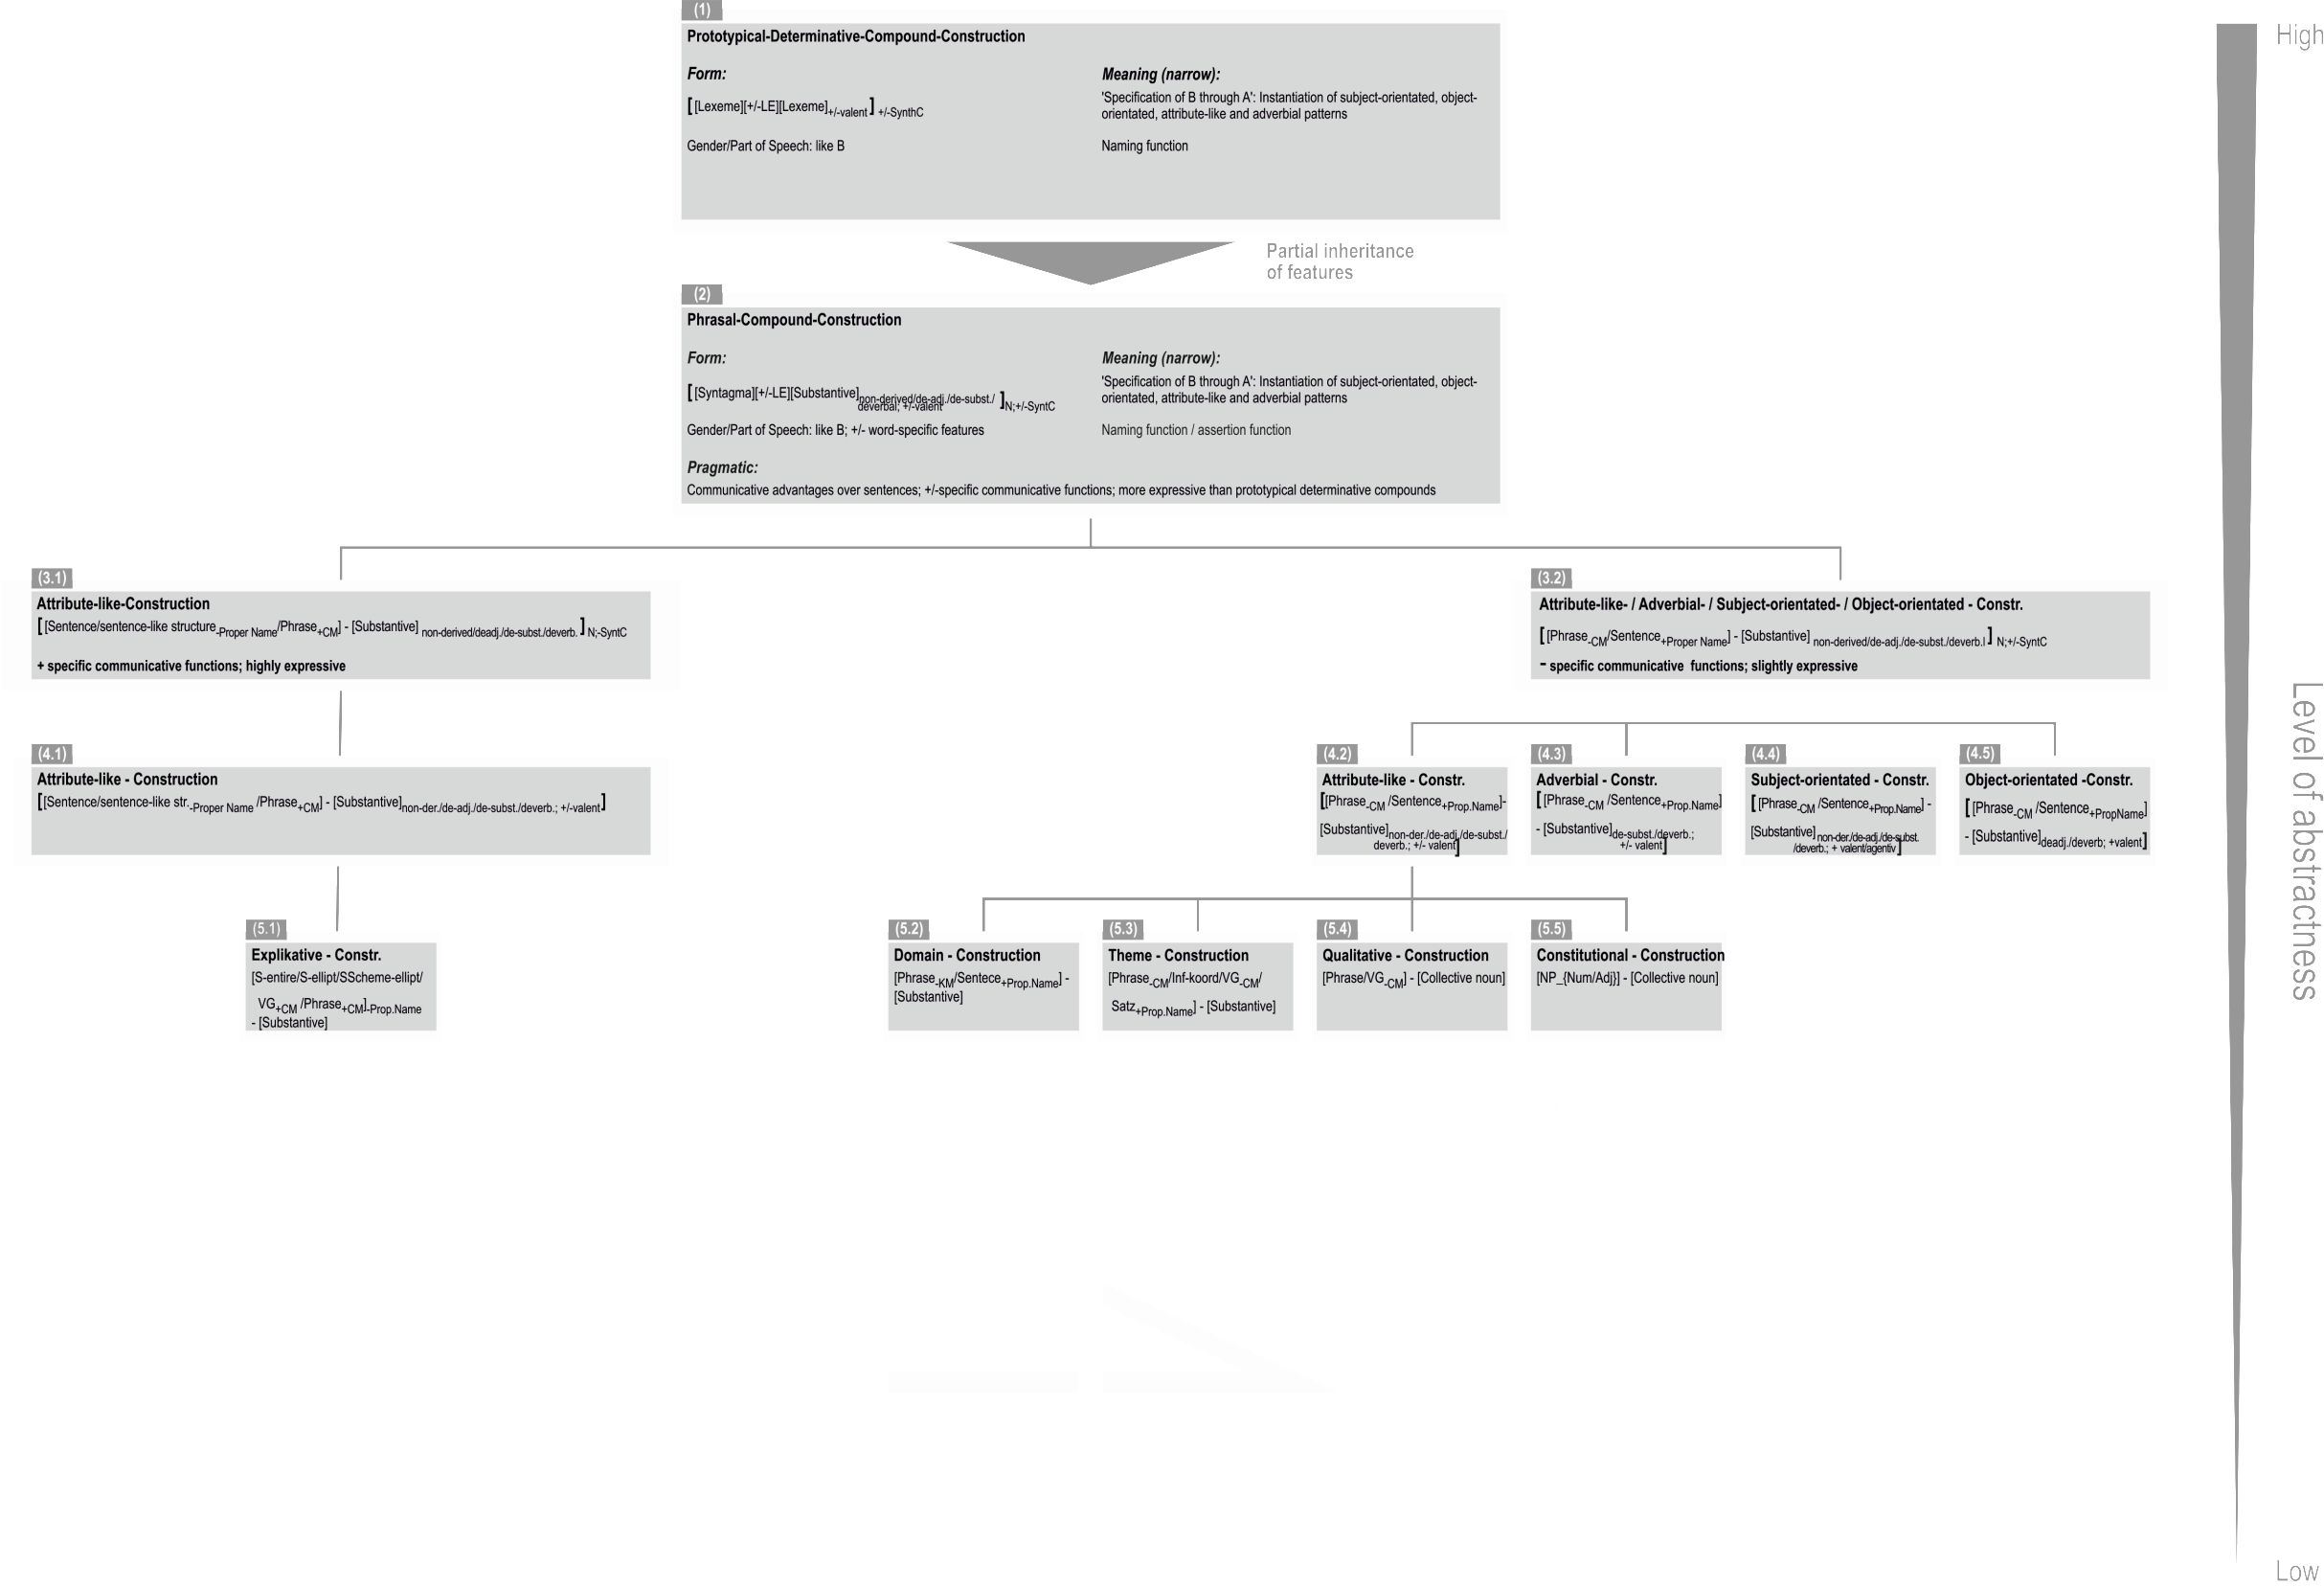
\includegraphics[width=\textwidth]{figures/ch5finalversionHein-img1.png}
\caption{``PC-Constructicon''}
\label{fig:hein:3}
\end{sidewaysfigure}


At the next level (3), the empirical observation that phrasal compounding can be split into two more specific patterns is integrated\footnote{However, phrasal compounding is also representable through one mutual form-meaning pairing on a more abstract level (2).}: I implemented that compounds with a sentence\slash a sentence-like structure or a phrase with the status of a CM as a first constituent (level 3.1) behave fundamentally different than compounds whose first constituent is built by a phrase without CM-status or a sentence which is a proper name (level 3.2). Both constructions at the third level inherit the central properties of the general PC-construction at level 2, but they are more concrete insofar as the \isi{syntax} of the first constituent, the type of meaning and such pragmatic properties that are not likewise displayed in all PCs are concretized. 



At level 4, the \isi{derivation} type of the head noun and its valence \isi{grammatical} properties are specified in addition. For example, at this level it is fixed that \isi{adverbial} readings are blocked in PCs with a deadjectival or a non-derived nominal head (cf. \figref{fig:hein:1.6} in \sectref{sec:hein:3.1.2}).


The constructions at level 5 (``explicative'', ``domain'', ``theme'', ``qualitative'', ``constitutional'') correspond to those frequent, universal form-meaning correlations which -- in part -- have been discussed in \sectref{sec:hein:3.1.1}.  In contrast to the constructions at levels 2 to 4, they do not cover the complete formal and semantic potential of phrasal compounding.  Instead, they represent only those correlations between form and meaning which are particularly well established.\footnote{It is striking that all constructions at level 5 are instantiations of the rough pattern ``attribute-like''. For the other  three rough patterns, no form-meaning pairings that are just as well-established can be stipulated.  This corresponds to the observation stated in \sectref{sec:hein:3.1.2} that in PCs attribute-like readings are the most common.} 



In the preceding paragraphs, I have provided an insight into the complex taxonomy that has been developed in \citet{Hein2015} by presenting a shortened and simplified version of the constructions found in my data\footnote{For example, I omitted the three most specific levels of the original taxonomy. Moreover, the important question how some ‘singular cases‘ can be integrated into the constructicon is not discussed in this paper (cf. \citealt[Chapter III.3.1.4.2]{Hein2015}.}. 



In conclusion, the ``dynamic'' of the constructicon has to be explained -- even if I do not claim ``psychological reality'' in the sense of carving out a one-to-one reproduction of the mental representation of phrasal compounding. 

Being confronted with a PC, the recipient initially tries to interpret it according to the most established form-meaning pairings of the constructicon. The recipient thus is aware that for a PC with a non-derived head noun, an attribute-like or a subject-orientated meaning is the most expectable (cf. level 4 of the constructicon).  In case that the received PC is not in accordance with one of those well-established readings,  the recipient falls back on a more abstract pattern of the constructicon (cf. level 3) and adjusts the received complex word with the interpretation potential offered at this level. 

Similarly, the producer of a PC is aware which semantic goals are typically realizable through the use of a certain formal type of PC, e.g. through the use of a PC with a non-derived noun in head position. In case the intention of the speaker\slash writer cannot be brought in line with the quite  specific, established form-meaning correlations at level 4,  he falls back on a more abstract pattern that represents that basically each of the four ``rough patterns'' is instantiable in PCs. 


\section{Conclusion}\label{sec:hein:4}
All in all, the empirical practicality of the conducted \isi{bottom-up process}, e.g. the possibility to structure the inventory of the 1,576 analyzed PCs with the help of pairings of form and meaning at varying degrees of abstraction, indicates that the properties of this word-formation type can be captured adequately through the mechanisms of \isi{construction grammar}. 

Looking at the frequency and the productivity of PCs, it is also justified and plausible in theoretical terms a) to ascribe them the theoretical status of a construction within a \isi{usage-based} model and b) to assume their \textit{mental} representation based on constructions. 

While PCs have the status of a marginal phenomenon in traditional generative approaches (cf. \citealt{Meibauer2003}, \citealt{Hein2011}) and should not even exist according to some of these approaches, I carved out a \isi{usage-based} model that can explain the functioning of the word formation pattern of phrasal compounding.

Finally, my paper highlights the degree to which a \isi{constructional} perspective provides interesting and new insights into the properties of the word-formation type examined here: As the conducted \isi{bottom-up model} takes the formal and semantic properties of the \textit{second constituent} as its starting-point, I argue that the properties of the head are the key through which the inventory of PCs can be systematized on the first level -- and not the abstract syntactic properties of the first constituent.

Last but not least, the approach presented here should be understood as an attempt to show ``how the notion ``construction'' can be made fruitful for morphological analysis and theorizing'' \citep[1]{Booij2010}.

\section*{Acknowledgements}

This paper is based on the findings of my doctoral thesis \citep{Hein2015}. Special thanks go to Gerd, Anette and Max Horten for improving my \ili{English}.

{\sloppy
\printbibliography[heading=subbibliography,notkeyword=this]
}

\end{document}